% Chapter 1

\chapter{Research And Design} % Main chapter title

\label{ResearchAndDesign} % For referencing the chapter elsewhere, use \ref{ResearchAndDesign} 

\section{Cooperative Governance}
\label{subsec:CooperativeGovernance}
The objective of this section is to outline the current processes surrounding cooperative governance, identify points of friction that are likely to arise as these processes are scaled and finally, to propose ways an Ethereum based application could provide solutions.

\subsection{Current Governance Model}
The best points of reference for understanding the current governance model of co-operatives are governing documents. Every cooperative has a set of governing documents which lay out the constitution and bylaws of the organisation. They are important in ensuring the overall direction, supervision and accountability of the cooperative. In plain terms governing documents help to establish: what the coop will do, who will do it and how they will do it. \\

The main topics covered in a set of governing documents are: membership, democracy, voting, general meetings, dissolution, administration, application of profits and dispute resolution. Because many cooperatives have similar governance requirements and take on a similar form, size and/or sector, there are a number of 'model rules' available to startup coops. For example, the trade organisation, Cooperatives UK \cite{modelRules} and Somerset Cooperative Services\cite{somersetRules} (SCS) both provide sets of model rules. The following subsections describe the main elements of cooperative governance as commonly defined within governing documents.\\

\subsubsection{Membership}
Co-operatives traditionally have been established to serve the specific interests or needs of a certain class of stakeholders, such as workers or consumers, however, each membership group has a different relationship to the cooperative entity. The first principle of cooperation, "voluntary and open membership", is interpreted within this context. A worker cooperative (for example, Suma\cite{Suma} with some 200 members) whilst having an open, non-discriminatory membership policy will also have a set of selection and appointment criteria for employees who wish to become members.  A consumer cooperative (such as, The Cooperative\cite{TheCoop}, 7m members) will have much less restrictive membership conditions: most individuals can become stakeholders by filling out a form and shopping at the group's stores.  A recent development has been the creation of Multi-stakeholder Cooperatives (MSC) that opens up membership to different classes of stakeholder: workers, consumers, users, investors etc through the use of the SCS's Somerset Rules.\\

Beyond defining stakeholder boundaries most governing documents also specify a minimum age for members (usually sixteen), a fee or minimum share purchase, the value of shares any member may hold, member commitments to governance and conditions for member termination.\\

\begin{figure}
\centering
\makebox[\textwidth][c]{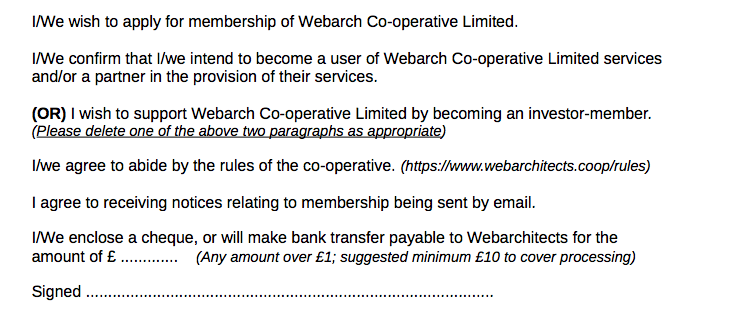
\includegraphics[width=1.4\textwidth]{Figures/webarchForm}}
\decoRule
\caption[Webarchitect's Membership Form]{A section of a membership application form for Webarchitects multi stakeholder cooperative illustrating example conditions of membership}
\label{fig:webarchForm}
\end{figure} 
Figure \ref{fig:webarchForm} is an extract from the membership application form for Webrarchitects\cite{webarchitects} (a multi stakeholder co-operative). Besides providing general personal information such as name, email and address, prospective members must also sign up to rules or conditions of membership.\\

\subsubsection{General Meetings}
General meetings (GMs) are the 'sovereign body' of a cooperative. Although any member may propose a resolution at a GM, the main focus is normally the election of directors and/or deciding on the application of profits. Co-operatives have a main annual general meeting (AGM) as well as several other general meetings throughout the year. Figure \ref{fig:workerCoopGM} shows an extract from the Coops UK Worker Co-operative Model.\\
\begin{figure}
\centering
\makebox[\textwidth][c]{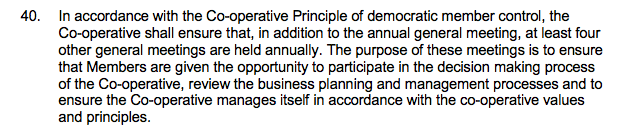
\includegraphics[width=1.4\textwidth]{Figures/WorkerModelGM}}
\decoRule
\caption[Worker Coop General Meeting Definition]{A section of the Coops UK worker co-operative model rules outlining the purpose of general meetings}
\label{fig:workerCoopGM}
\end{figure} 

General meetings may be called at the discretion of the board of directors or following a demand from a set threshold of the membership. For example, the worker co-op specifies the lesser of one tenth of or 100 members.

\subsubsection{Board of Directors}
A board of directors is a subset of the membership in large co-operatives, appointed to manage the business of the cooperative and who typically have the right to exercise any powers that might be exercised by the cooperative as a whole. It is important for the survival of the co-operative that directors have sufficient competence to effectively and efficiently manage the business. Some co-operatives pass standing orders to define the necessary skills and qualifications for director positions.

\subsubsection{Voting}
\begin{figure}
\centering
\makebox[\textwidth][c]{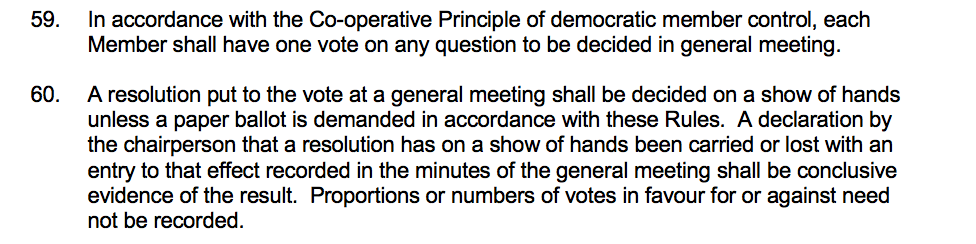
\includegraphics[width=1.4\textwidth]{Figures/WorkerRulesVoting}}
\decoRule
\caption[Worker Coop Voting Process]{A section of the Coops UK worker coop model rules illustrating an example voting process.}
\label{fig:WorkerRulesVoting}
\end{figure} 
Co-operatives are almost always 'one member one vote'. The voting process in small cooperatives may just be a show of hands. Large member coops must have sophisticated member engagement strategies to inform, encourage and enable members to take part in postal or online ballots to elect directors or pass important motions. Figure \ref{fig:WorkerRulesVoting} shows the main voting clauses from the Coops UK worker co-operative model rules. Voting in multi stakeholder cooperatives can be slightly more interesting as the rules must protect against unfair representation or dominance of a single stakeholder group. Figure \ref{fig:SomersetVoting} shows an extract from the Somerset Rules. The Somerset rules also specify that no resolution may change the rules on class weighting themselves. 
\begin{figure}
\centering
\makebox[\textwidth][c]{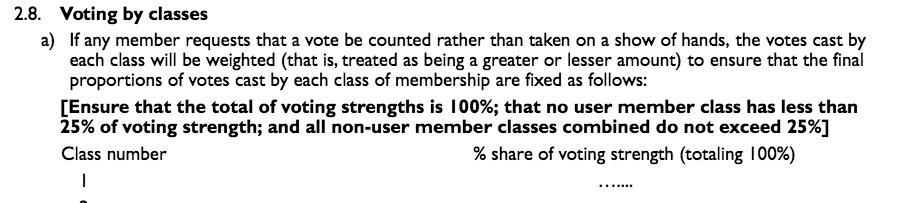
\includegraphics[width=1.4\textwidth]{Figures/SomersetVoting}}
\decoRule
\caption[Somerset Rules for Class Based Voting]{A section of the Somerset multi stakeholder model rules illustrating the complex and contractual nature of class based voting.}
\label{fig:SomersetVoting}
\end{figure} 

\subsubsection{Quorum}
A quorum simply defines the minimum number of members that must be present at decision making meetings in order to carry out business. Its purpose, like that of voting thresholds (such as, "two thirds majority") for changes to key parts of the constitution, is to safeguard the organisation from control or dominance by unrepresentative groups or decisions.

\subsubsection{Resolutions}
A resolution or motion is a formal proposal to change some aspect of the organisation's behaviour or practice. High level decision making works through proposing and voting on resolutions. Normally governing documents make a distinction between normal and extraordinary resolutions and the proportion of the vote required to pass the resolution. Normal resolutions are typically non-constitutional and require a lower majority. Extraordinary resolutions are often constitutional and propose changes to the rules of the cooperative itself. Some co-operatives choose consensus decision making and require 100\% agreement on all resolutions.

\subsection{A Scalable Governance Solution}
For most co-operatives, the tried and tested governance models described above are very effective. The problem which has been identified in the motivation to this study, however, is that when scaled, they become less efficient and less effective at representing the membership: barriers are created by membership numbers, spatial distribution and time -  to attend meetings and/or understand the issue.  The systems put in place to overcome these problems traditionally have been "representative" based branch and regional meetings, postal and online balloting, all of which create considerable friction to membership participation. This is illustrated by The Cooperative group where, despite the Mynors led overhaul\cite{Myners} of the governance architecture, low participation remains problematic as the Interim Results of the Group, 4, July, 2015 conclude:\\

"The fledgling nature of the new democratic structures was reflected in voter turnout at the AGM, with  3\% of eligible members casting their votes. Our ambition is to see this number substantially increase as we implement our member engagement programme, which will launch in mid-2016. This aims to reverse many years of declining member participation."\cite{CoopParticipation}\\

The following subsections describe how an Ethereum based application might address scaling issues faced by the various elements of governance.\\

\subsubsection{Membership}
Large co-operatives store membership details and attributes in databases. These provide the basis on which the organisation carries out "member relationship management" functions, more typically termed customer relationship management, that is, enroll and validate membership identity and credentials, carry out communications, store transaction details, surveys and conduct postal or online ballots etc.  The creation, storage, configuration and use of this data must comply with UK law as set out in the Data Protection Act\cite{DataProtection}: 
\begin{itemize}
\item used fairly and lawfully
\item used for limited, specifically stated purposes
\item used in a way that is adequate, relevant and not excessive
\item accurate
\item kept for no longer than is absolutely necessary
\item handled according to people's data protection rights
\item kept safe and secure
\item not transferred outside the European Economic Area without adequate protection
\end{itemize}

The data holder in this instance must have considerable organisational competence to manage this information. A trusted relationship emerges between the members and the data holder, in this case an organisation over which the members have democratic control and scrutiny.\\

There are a number of ways the Ethereum platform can aid the legal compliance of a governance application:
\begin{itemize}
\item Public private key authentication means that access to data can be restricted to only permissioned key holders. This offers a much higher level of cryptographic security than many existing systems. Encryption of data on the blockchain is discussed further in section \ref{sec:blockchainprivacy}.
\item Member information does not need to be held by every individual co-operative. It can be stored in the blockchain once where it is controlled by its owner. This makes it much easier to keep data accurate and secure.
\item The resilience and high availability of the peer to peer network mean data is safe from damage or disaster.
\end{itemize}

Further to this, Ethereum's corruption resistant nature and the transparency of contract code mean a governance application can establish a high level of trust with members. Members can be uniquely identified by an Ethereum account (discussed further in section \ref{sec:identity}) which makes it easy to collect membership fees in Ether and enforce secure voting.\\

\subsubsection{General Meetings}
General meetings create practical spatial and temporal barriers to member participation - people have to make a considerable effort to be in the right place at the right time to engage in the discussion and the decisions, this naturally discriminates against anyone who is unable to travel or cannot attend at a particular time.  When coops are small, localised or workplace based this is not a significant issue.  When coops are large and/or distributed general meetings tend to become representative of the members who have the time and resources etc to take part. Location, distance, time, cost etc increase barriers to participation. General meetings to some extent could be characterised as an artifact of the pre-web era but despite the widespread adoption of digital decision making tools, such as Loomio (see \ref{subsec:RelatedWork}), they still form a central pillar of co-operative governance. There are a number of possible reasons for the "live" F2F (face to face) GM's popularity, including: the quality of the abstracted online communication - loss of immediacy; lack of technical competency to set up digital systems and lack of trust in the security and auditability of these tools. \\

The business - structured list (agenda) of decisions to be taken - at a General Meeting typically will comprise:
\begin{itemize}
\item documentation with a valid and verifiable origin within the organisation, that is, put forward by a legitimate body or members according to the standing orders,
\item a deliberative process where arguments for the proposal are set out and discussed, amendments can be made and the final wording of the motion put to a vote or poll.
\end{itemize}

There are three key aspects to this process:\\

Firstly, the ability of the participants to "be in the room", have sight of the proposal, see and hear the deliberations, have the opportunity to speak or suggest amendments.  \\

Secondly, the documentation of a resolution and the final form must be accurately configured to reflect the amendments (transactions) to be put to the vote, and \\

Thirdly, the rules or standing orders must be understood and followed by either the live or the digitally enable processes.\\

A range of applications may be used to overcome the spatial and temporal barriers and recreate the real world experience and processes used in GMs, for example, streaming video and audio (citrix), text based exchanges (Loomio) and possibly in the future Virtual Reality Headsets, if these become widely available. The role of an Ethereum application would be to deal with configuration management - recording and tracking changes (versions of the proposal), establishing the final form of words that will be put to the vote and the voting process itself (following appropriate rules defined by a co-operatives standing orders). Such an application would offer similar functionality to tools such as Loomio but with security guarantees that make it usable for binding decisions. \\

An Ethereum based application could therefore fulfill the requirements of the decision making process currently facilitated by GMs whilst simultaneously offering a high enough level of trust and security to enable its adoption. Costs could be reduced whilst participation and efficiency are increased. The ability to make decisions collectively is no longer restricted by the logistical constraints of organising physical real world meetings.\\

\subsubsection{Resolutions}
Proposals or resolutions must be documented and be capable of dynamically changing in response to amendments in a General Meeting scenario. An Ethereum application could enable digital collaboration whilst permanently versioning changes to proposals into the blockchain. A smart contract system could trivially render a final form immutable and make it available to everyone with valid voting credentials. In addition, many constitutional or extraordinary resolutions passed by a co-operative could be implemented by the smart contract system itself. For example, the normal resolution level of a co-operative must be stored in the smart contract system in order to implement a correct voting algorithm. Executing a proposal that changes the normal resolution would therefore be as simple as changing a variable within a program!\\

\subsubsection{Voting}
At the point of voting on a proposal it is necessary to accurately record that valid votes are cast, that is, by members entitled to vote, that a result of the vote is accurately recorded and can be audited should that be required.  Clearly counting hands doesn't scale, neither is it private or easily verifiable and is subject to the human error of the "tellers". Paper based ballots and postal voting where the whole membership is required to vote can scale, but become costly, unwieldy, slow as well as creating friction to participation.  The prospect of electoral fraud may be of less significance in organisational ballots where there is little to be gained personally by individuals but any system should be sufficiently robust that fraud is guarded against.\\

A voting system based on Ethereum has the potential, through the use of smart contracts using transactions signed with verified public-private keys, to digitally enable whole member votes to be deployed securely and rapidly across a widely distributed membership. This does depend on members being willing to use the internet and the distributed applications. Many of the voting rules, such as those shown in figure \ref{fig:SomersetVoting}, lend themselves naturally to the kind of logic that can be embedded in a smart contract system. \\

\subsubsection{Quorum and Thresholds}
Quorum and thresholds can be designed into smart contract systems to ensure the vote is valid in accordance with agreed rules. The system can be designed to automatically "defeat" or pass any resolution that does not reach the threshold at the closing date.\\

\subsubsection{Boards}
Unlike general meetings, the existence of directors is less a product of available technology and more concerned with efficient operation. Not all decisions need to be taken at the level of the cooperative, that is, by the full membership or General Meeting. Even within large distributed cooperatives directors will be required to manage operational matters. \\


\section{Privacy on The Blockchain}
\label{sec:blockchainprivacy}
Ethereum is a permissionless blockchain. This means any peer can freely join the network and participate in the mining process. The security of Ethereum is reliant on the ability of any of these peers to validate the correct linking of, and state transitions between, all blocks in the history of the chain. This group consensus is what makes blockchains so valuable but it is also the reason why the whole blockchain must be publicly visible (at least to the permissioned set of peers). If it were possible to censor parts of the chain or hide certain transactions then the validation process would break down and all trust in the network would be lost. In Ethereum this means any call to contract code, any change in contract state or any transfer of ether is transparent. This is a fairly obvious point but worth making because it is easy to lose sight of the basic when dealing with the complex.\\

The transparency of the Ethereum blockchain introduces a couple of obstacles for application developers. The first one is how private data should be managed. The second, and slightly more complex, is how computations that require the input of private data can be executed. This section introduces some possible approaches to tackling these issues both of which are relevant to the development of Go-op. \\

\subsection{Storing Private Data}
As discussed in \ref{subsec:CooperativeGovernance} , a likely requirement of Go-op is the protected storage of membership information. Cooperative members should have access to the personal information of other members but such information should not generally be accessible to any other party. \\

Private data can be stored on a blockchain by simply encrypting it first. The ciphertext will be publicly visible but the information will be hidden. An Ethereum account address is derived from the public key of a public-private key pair generated using ECC (Elliptic Curve Cryptography) and the SECP-256k1 curve parameters (described in the Yellow Paper \cite{wood2014ethereum}). Taking advantage of these key pairs, encryption of member information could potentially be achieved as follows:\\

For each intended recipient of the data:\\
\begin{enumerate}
\item Retrieve a public key from their public address. Possible using the Solidity ecrecover function\cite{SolidityCheatsheet} or in the browser (manually\cite{StackExchangeAddress} or using a library\cite{WalletJS}).

\item Use the public key to encrypt the data in the browser using ECC asymmetric encryption.

\item Store the ciphertext in the Ethereum blockchain.

\item Recipients read from blockchain and decrypt using their private key (obtainable from their address following similar process step 1) 

\end{enumerate}

A nice aspect of this approach is that it doesn't introduce any additional key management complexity and by taking advantage of the 'Web3.0 architecture' (see section \ref{sec:web3Arch}) the process can also be simplified somewhat. The ciphertext can actually be stored in a distributed file system (such as IPFS see  \ref{subsec:ipfs}) and a link (e.g. IPFS hash) can be stored in the blockchain instead. \\

Asymmetric encryption techniques such as ECC however, are fairly computationally intensive which could make this approach unwieldy in the face of thousands of users. More importantly, asymmetric encryption schemes are not generally recommended for encrypting large messages and are instead used for the secure exchange of symmetric keys. This form of hybrid approach is thought to be more secure and efficient. For encryption on Ethereum, such a process might look like the following:

\begin{enumerate}
\item Generate a symmetric key. 
\item Encrypt data with symmetric key (e.g using AES).
\item Store the encrypted data (or IPFS address of encrypted data) in the blockchain.
\item For each intended recipient, encrypt the symmetric key following an asymmetric encryption method similar to the one described previously.
\item Store mapping of Ethereum accounts to matching ciphertexts of the symmetric key on the Ethereum blockchain (again this can be more efficiently stored in IPFS and referenced from blockchain)
\item Recipients read from blockchain to find a) the ciphertext of the data (step 3) and b) the ciphertext of the symmetric key (step 5)
\item Recipient decrypts the symmetric key using their private key and then decrypts the data using the symmetric key.
\end{enumerate}

This method still requires the same number of asymmetric encryption operations as before but the process is less computationally intensive because the size of the plaintext (i.e. the symmetric key) encrypted in this way is constant and much smaller. The encryption of any potentially large amounts of data only needs to be performed once using symmetric encryption.\\

Any change to the encrypted information is relatively easy to handle because, providing a suitable block cipher mode is chosen, the same symmetric key can be reused. Granting access to new accounts is also easy because it only requires one additional encryption of the symmetric key with the public key of the new account. The drawback is that whenever a key needs to be revoked, the symmetric key is compromised and any future encryption would need to repeat the whole process with a new symmetric key. From a security perspective, we must assume that any information encrypted with the old symmetric key is known to the excluded party, it is not possible to enforce forgetfulness. \\

Controlled access to information and privacy in general are common requirements for many applications. It is probable that, as the Ethereum ecosystem matures, more tools and solutions will become available to make this process easier and safer for application developers. \\

\subsection{Computing Private Data}
A more complex requirement than the storage of private information is performing computation with it. Consider anonymous voting, which is highly relevant to the Go-op application, where the objective is to calculate the outcome of a vote without revealing any information about the choices of individual participants. Calculating the result of a vote on Ethereum would make the process secure but, again, because execution of contract code is transparent, it makes it difficult to ensure privacy. A potential solution would combine some method of blinding a vote with a method for counting the blinded values.\\

Provable honest voting systems that protect voter privacy have been widely discussed\cite{PrivacyBlockchain}\cite{HonestElection}. Possible solutions include the use of ring signatures\cite{liu2004linkable}\cite{tsang2005short} and addition through homomorphic encryption\cite{HomoEncryption}.\\

\subsection{A Word on Solidity Access Modifiers}
Whilst the Ethereum blockchain is transparent, the Solidity language features various visibilities for functions and state variables (see figure \ref{fig:AccessModifiers}, so what does this mean? \\
\begin{figure}
\centering
\makebox[\textwidth][c]{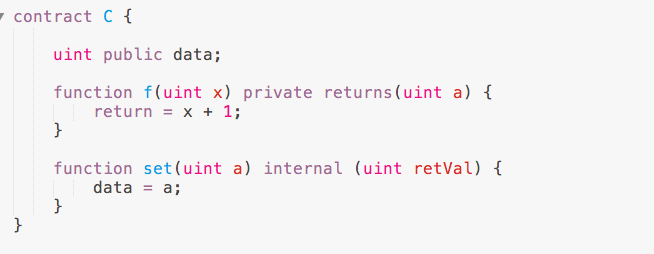
\includegraphics[width=1.4\textwidth]{Figures/AccessModifiers}}
\decoRule
\caption[Solidity Access Modifiers]{Illustration of various access modifiers for state variables and functions within Solidity}
\label{fig:AccessModifiers}
\end{figure}
Access modifiers within Solidity, like in many other languages, are designed to aid code encapsulation. Whilst they restrict the behaviour of executing contract code, and therefore help to catch bugs and errors at compile time, they don't provide any access modification to any external entity reading from the blockchain.\\

%%%%%%%%%%%%%%%%%%%%%%%%%%%%%%%%%%%%%%%%%%%%%%%%%%%
%%%%%%%%%%%%%%%%%%%%%%%%%%%%%%%%%%%%%%%%%%%%%%%%%%%
\section{Oracles And Identity Management}
\label{sec:identity}
For many real world and digital services the 'proof of identity' or KYC (know your customer) problem is very important. For financial service providers, knowing the customer can help to mitigate risk (issuing loans etc), avoid money laundering or protect against fraud. In any kind of democracy application such as Go-op, where we need to enforce the principle of 'one member one vote', identity management is key to fair representation and the avoidance of double votes.\\

The 'proof of identity' problem does not disappear when we move to the blockchain. Given that any Ethereum user can generate multiple accounts it is very tricky to identify an individual in a completely 'trustless' fashion. 

\subsection{e-Residency}
e-Residency is a transnational digital identity offered by the government of Estonia to any global citizen wishing to administer a location independent business online \cite{e-Residency}. To become an e-Resident applications must provide a photo ID and a copy of their pre-existing government issued identity (such as a passport). A background check is then conducted by Estonian officials before the applicant is able to collect the card, in person, to verify their identity. In return, e-Residents receive a smart ID card with a unique public private key pair that both proves the identity of a person and allows them to easily create digital signatures. Technically, digital certificate chains are used to prove that the key-pair within the e-Resident card are derived from a key-pair controlled by the Estonian government. \\

\begin{figure}
\centering
\makebox[\textwidth][c]{\includegraphics[width=\textwidth]{Figures/e-Residency}}
\decoRule
\caption[e-Residency Card]{e-Residency card issued by Estonian Government}
\label{fig:e-Residency}
\end{figure}

Returning to the 'proof of identity' problem on Ethereum, e-Residency provides a way for the Estonian government to become the trusted authority on the identity behind an Ethereum account (see \cite{IDBereg} \cite{BertaniKYC} for more on this idea) but there are still a few barriers to practical implementation. Firstly, e-Resident cards use RSA encryption. Verification of RSA signatures 'on-chain' is not yet possible although this could well change in the future \cite{RSARequest}. Secondly, the Estonian government would need to engage with Ethereum and publish their top level certificates to the blockchain so that other contracts can use them for signature verification. Given their commitment to e-Residency and history in pioneering technical solutions\cite{EstoniaE-Voting}, this doesn't seem too improbable. A temporary work around could be the use of a trusted 'oracle'\cite{BertaniOracles}, such as Oraclize\cite{Oraclise}.

\subsection{Curators}
TheDAO (briefly explained in \ref{subsec:DAOs}) is an Ethereum based organisation that is able to subcontract work to external, real world entities. Proposals for work are submitted to TheDAO as smart contracts and members vote to accept them. However, without knowing the identity of contract proposers, members have no idea whether proposals are legitimate, and therefore likely to be completed, or just spam. In general, the operation of TheDAO will be more efficient if the identity of service providers is known.\\
 
To solve this identity problem TheDAO introduces the concept of a 'curator'\cite{TaulCurators}. One of the main roles of a curator is to validate that any contractor who makes a proposal is a real person or organisation. This is an off the chain process that requires TheDAO members to trust the curators. Members of TheDAO can, at any time, vote to replace curators but the requirement for a trusted third party still remains.\\

This is a more localised approach to trust than e-Residency. The e-Residency card has the potential to form a general identity provision infrastructure that could be used by any Ethereum service. Managing identity this way would require all users of your application to be e-Residents. In contrast, the approach taken by TheDAO simply requires the election of a trusted member to validate identities 'off-chain' but any identification here is unlikely to pass muster within other organisations. \\


%%%%%%%%%%%%%%%%%%%%%%%%%%%%%%%%%%%%%%%%%%%%%%%%%%%
%%%%%%%%%%%%%%%%%%%%%%%%%%%%%%%%%%%%%%%%%%%%%%%%%%%

\section{Blockchain Time}
\label{sec:blocktime}
There are a couple of interesting design challenges surrounding smart contract applications that need to work with time. Firstly, how can accurate and reliable time measurements be accessed within the blockchain? Secondly, how can contract code react to an event at a specific time? For a governance or democracy application measuring time is important for closing ballots at the correct date. Ideally we would like an accurate notion of time (to make things as fair as possible) that we can react to in order to prevent further voting and to calculate the result.\\

\subsection{Accurate Timestamps}
For a block to be accepted by a miner, the state transition function has to produce the same output as it did for the block creator. If smart contract code used the host machine's (i.e. miners) system time for its logic then this could easily \keyword{not} be the case because blocks are not created and validated at the same time. The only time reference that can be used, because it is consistent, is the timestamp of the block a transaction is included in. Ethereum smart contracts written in Solidity can access this time easily through the \code{block.timestamp} property. The problem with the block timestamp however, is that it is not necessarily accurate. The Ethereum protocol places some restrictions on timestamps but cannot be too strict because it must accommodate for drift in clocks across the network. Whilst this may be a cause for concern in highly time critical applications, in reality, the block timestamp is probably accurate enough for most usages.\\

\subsection{Scheduled Execution}
Unfortunately, because smart contract code can only be executed as the result of an external transaction and cannot simply 'wake up', the ability of contracts to schedule execution or react to time based events is limited. There are two possible solutions for smart contracts that need to execute code based on the time - eager and lazy evaluation. \\

A contract working eagerly will somehow arrange for an external transaction to call its evaluation code at a specific time in the future. In contrast, a contract working lazily will just wait for a transaction to occur 'naturally' and then, if the time of an event has passed, evaluate it's logic.\\
\begin{figure}
\centering
\makebox[\textwidth][c]{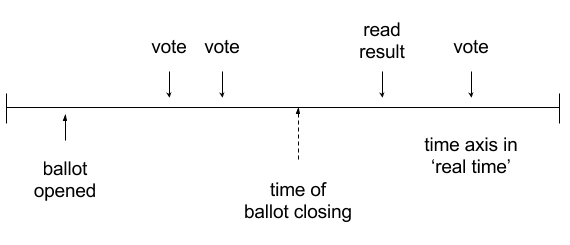
\includegraphics[width=1.2\textwidth]{Figures/lazy}}
\decoRule
\caption[Lazy Contract Scheduling]{Timeline of ballot contract calls with lazy evaluation}
\label{fig:lazy}
\end{figure}

Figure \ref{fig:lazy} shows an example time frame for a ballot contract. When the ballot closes the contract may need to perform some additional logic to calculate a result or close the voting. Following a lazy approach, this is triggered by the 'read result' transaction which is the next transaction to occur. There are a couple of issues with the approach. Firstly, if no transactions 'naturally' occur after the ballot closes then the evaluation simply can't happen. Secondly, the 'read result' method must become a transaction because it might trigger evaluation code which updates state in the blockchain. Ideally, getting the result should just be a call and the first user to ask for it shouldn't have to pay!\\

To address these problems an 'eager evaluation' solution has been developed by the Ethereum community called the Ethereum Alarm Clock\cite{EthereumAlarmClock}. For a small fee, the Ethereum Alarm Clock service allows contracts to schedule calls by registering their address and the definition of a function they would like to be executed. The Ethereum Alarm Clock service uses this payment to offer a bounty to any user account that makes the transaction at the scheduled time. The service creates a marketplace for function calls that any Ethereum user can participate in. Figure \ref{fig:eager} shows how a ballot would be closed using the Alarm Clock service.\\

\begin{figure}
\centering
\makebox[\textwidth][c]{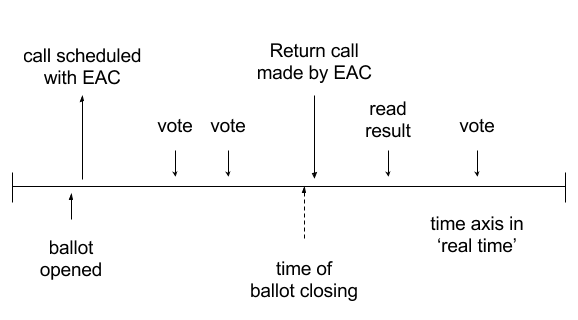
\includegraphics[width=1.2\textwidth]{Figures/eager}}
\decoRule
\caption[Eager Contract Scheduling]{Timeline of ballot contract calls with eager evaluation}
\label{fig:eager}
\end{figure}
The eager evaluation solution also has its flaws. Firstly, calls are scheduled for a given period of blocks into the future and not at a given time. Secondly, the service cannot guarantee that a call will be executed. It relies on an open market of rational actors but if no one wants to collect the fee for your function call then it cannot happen.\\

%%%%%%%%%%%%%%%%%%%%%%%%%%%%%%%%%%%%%%%%%%%%%%%%%%%
%%%%%%%%%%%%%%%%%%%%%%%%%%%%%%%%%%%%%%%%%%%%%%%%%%%
\section{Idealised Web3.0 Architecture}
\label{sec:web3Arch}
Dr Gavin Wood, author of the Ethereum yellow paper\cite{wood2014ethereum} and lead developer of the c++ client, gave a talk at a Meetup in 2014 called 'The Ethereum Experience' (video\cite{Web3Vid} and slides\cite{Web3Slides} available) in which he outlined an idealised architecture for Web3.0 applications. In addition to Ethereum, Wood presents two complementary technologies (also developed by the Ethereum foundation) called Whisper and Swarm.\\ 

Swarm is a distributed file system that is very similar in nature to IPFS (see \ref{subsec:ipfs})\\

Whisper is a private and public messaging system built into Ethereum. Conceptually it is something akin to UDP (User Datagram Protocol) and enables dapps to communicate through instant transient messaging. Whisper uses probabilistic routing, high levels of encryption and is subscription based, meaning messages can easily be filtered.\\

Together, Ethereum, Swarm and Whisper form a complementary stack of tools for building completely distributed web applications.\\ 
\begin{figure}
\centering
\makebox[\textwidth][c]{\includegraphics[width=1.4\textwidth]{Figures/DappArch}}
\decoRule
\caption[Idealised Web3.0 Architecture]{Idealised Web3.0 architecture. Diagram taken from the Ethereum Experience \cite{Web3Slides}}
\label{fig:DappArch}
\end{figure}

Figure \ref{fig:DappArch} is a conceptual diagram showing the interaction of three dapps in an idealised Web3.0 architecture. The green circles represent client computers, perhaps even a single program such as the Mist browser. The 'backend' of the dapp consists of logic split between javascript running in in the browser and the Ethereum blockchain. Dapps communicate dynamically using Whisper for public and private instant messaging and Swarm for file or content storage.\\
\begin{figure}
\centering
\makebox[\textwidth][c]{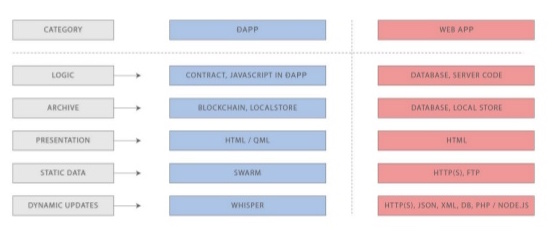
\includegraphics[width=1.4\textwidth]{Figures/DappVWeb}}
\decoRule
\caption[Web App v Dapp]{Dapp and traditional 'web app' comparison. Diagram taken from the Ethereum Experience \cite{Web3Slides}}
\label{fig:DappVWeb}
\end{figure}
\\
The process for loading a dapp in this system might go something like the following:\\
\begin{enumerate}
\item User opens their Web3.0 enabled browser such as Mist.
\item User searches for app in navigation bar e.g eth://go-op
\item A top level DNS contract in Ethereum returns address of static files for Go-Op front end within a distributed file system such as IPFS.
\item Mist browser fetches web app from distributed file system and renders it.
\end{enumerate}

\subsection{Status}
This is an idealised architecture because its components do not yet fully exist. Ethereum is currently at 'Homestead', one of the several milestones in a security led release process\cite{VinayLaunch} (we are still waiting for official release of Mist and Casper proof of stake protocol for example). According to Victor Tron (Ethereum core developer), both the go and c++ Ethereum clients have fully functional Whisper implementations\cite{TronStack}. However, other than a short section in the Web3 API, Whisper is not widely documented and at this point hardly appears in any community or official documentation.\\

Swarm is still under development by the Ethereum go team. At the time of writing they are working closely with IPFS to try and integrate the two projects\cite{DevUpdate}. \\

%%%%%%%%%%%%%%%%%%%%%%%%%%%%%%%%%%%%%%%%%%%%%%%%%%%
%%%%%%%%%%%%%%%%%%%%%%%%%%%%%%%%%%%%%%%%%%%%%%%%%%%
\section{Smart Contract Design Patterns}
\label{sec:scDesign}
Smart contract backends for distributed applications are typically composed of multiple components - "Every non-trivial DApp will require more than one contract to work well. There is no way to write a secure and scalable smart contract back-end without distributing the data and logic over multiple contracts."\cite{FiveTypes}\\

Although smart contracts might be thought of in a similar way to normal web services (they provide a public facing API at a specific address over a network) there are many differences that make the process challenging and demand special attention. \\

The first of these is the immutability of contract code. The code of an Ethereum contract account cannot be changed and is therefore bound to the account address. This implies that if we want to evolve smart contract systems over time we either have to redeploy them or design them in a highly modular fashion. Modular systems are generally the prefered option because it minimises costs, prevents blockchain bloating and maintains the same access address for service consumers. \\

Another challenge for smart contract systems is permission management. Ethereum applications are generally required to be secure. If a system grows into multiple contracts then besides modularity, contracts need to know who is calling them and what level of permissions they have. \\

This section introduces a couple of useful patterns to aid smart contract development.\\

\subsection{Events}
\label{subsec:events}
Front end dapp code uses the web3.js library\cite{Web3JS}, which exposes the Web3 Javascript API\cite{JavascriptAPI}, to interact with smart contracts. in turn, the web3 library communicates with the local Ethereum node through an RPC (Remote Procedure Call) interface. Depending on whether smart contract code modifies the blockchain (i.e changes contract storage state) a function call will either be a 'transaction' or a 'call'. Calls do not require gas to execute and a web3.js callback will be passed the same return value as the solidity function. Transactions however, need to be processed by the network. They require gas to execute and the argument passed to the callback is a transaction hash, not the return value of the solidity function. Return values for non-constant (state changing) contract functions are only returnable to calls from other contracts within the EVM not from an external call. A potential implication of this is that it becomes difficult for a dapp to know whether a transaction (i.e state changing function call) successfully completed or whether it failed (conditions, exceptions, out of gas etc). A simple design pattern that uses Ethereum events is used to handle this. \\
\begin{figure}
\centering
\makebox[\textwidth][c]{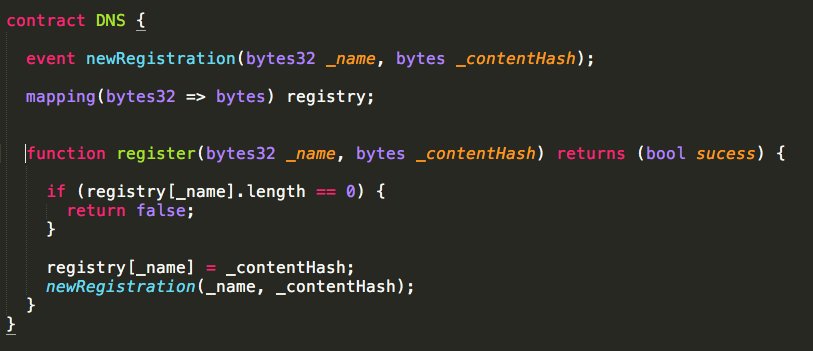
\includegraphics[width=1.4\textwidth]{Figures/DNSContract}}
\decoRule
\caption[Example DNS Contract]{A simple domain name registration contract to illustrate the use of events.}
\label{fig:DNSContract}
\end{figure}

Transaction logs are generated by Ethereum clients during contract execution (whilst they are not part of the consensus mechanism per se, transaction logs are verified by the blockchain because transaction receipt hashes are stored inside blocks). Events are an Ethereum feature that allow a contract to write to the log of the executing transaction. Dapps running in the browser can then subscribe to the logs of their local Ethereum client in order to receive notifications for particular events. Figure \ref{fig:DNSContract} shows some sample Solidity code for a simple domain name registration  contract. If a name is already registered then the function call 'fails' and simply returns. If a name is not yet registered then the contract adds a mapping for the associated content and fires an event. Dapp code can subscribe to the newRegistration event to find out whenever a new registration takes place. In fact, the web3 API actually allows filtered event subscritpion so dapp code could even just listen for a registration of a particular domain name. \\

\subsection{The Five Types Model}
The five types model is a smart contract system design pattern created by Eris industries\cite{FiveTypes}. It describes a modular architecture based around the concept of a contract management contract or CMC which acts as the authority or reference point for other system components. \\
\\
The five types of contract within this model are as follows: \\
\begin{enumerate}
\item \keyword{Database Contracts.} Data storage contracts that provide read, write and update functionality. 
\item \keyword{Controller Contracts.} Add layer of more complex behaviour to data storage operations. In a flexible system controllers and databases have APIs that allows them to easily be swapped in and out.
\item \keyword{Contract Management Contracts.} Keep track of all other contracts in the system as a mapping from component name to contract address.
\item \keyword{Application Logic Contracts.} Application specific code or business logic.
\item \keyword{Utility Contracts.} Library functions.
\end{enumerate}

\begin{figure}
\centering
\makebox[\textwidth][c]{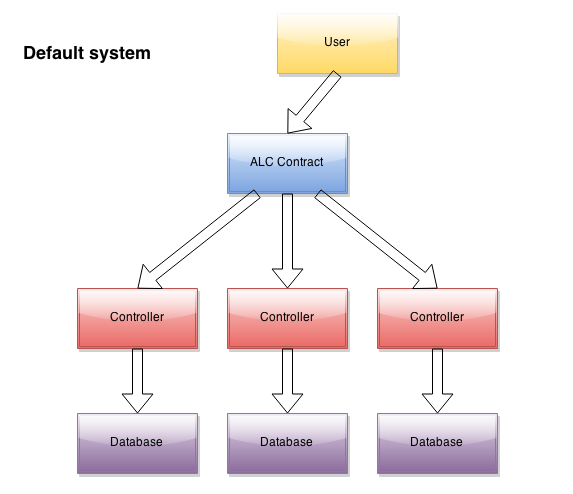
\includegraphics[width=\textwidth]{Figures/FiveTypesSystem}}
\decoRule
\caption[Five Types Dependency Graph]{Five Types component dependency diagram (original by Eris Industries \cite{FiveTypes}}
\label{fig:FiveTypesSystem}
\end{figure}

\begin{figure}
\centering
\makebox[\textwidth][c]{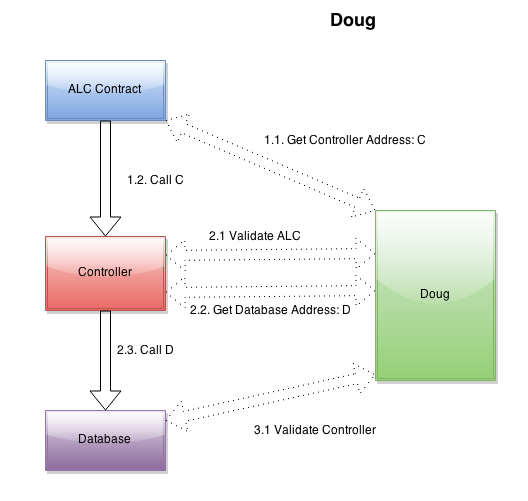
\includegraphics[width=\textwidth]{Figures/FiveTypesDOUG}}
\decoRule
\caption[Five Types Contract Management Contract Interaction]{Illustration of contract management contract (Doug) within Five Types model.}
\label{fig:FiveTypesDOUG}
\end{figure}

Figure \ref{fig:FiveTypesSystem} (taken from Eris industries tutorials - see ref) shows a dependency graph between different components of a generic smart contract system built following the five types contract design pattern. Figure \ref{fig:FiveTypesDOUG} (also taken from Eris industries tutorials) shows how various components within a five type model interact with one another including with the contract management contract (here called Doug). Contracts confer with Doug to both validate the address of the calling contract and also to retrieve the address of any other contracts they themselves need to call.

\subsubsection{Benefits}
The principle benefit of the Five Types design pattern is modularity. Before calling code from another system component every contract first confers with the CMC to retrieve the correct address. This means that so long as the existing API is still supported, a system administrator can update the CMC with new component addresses and the whole system will continue to work.\\

An additional benefit of the Five Types design pattern is permissioned access. The CMC makes it easy for contracts to check the identity of a calling contract and terminate execution if it is foreign or unauthorised. \\


\subsubsection{Critiques}
Modularity comes at a cost. By introducing extra calls and more processing, the Five Types pattern increases the cost of execution. Modularity also introduces a degree of trust. A modular system must give some agent(s) the power to to update the behaviour of smart contract system. Of course, from a technical standpoint any changes made to the system will be publicly visible but practically, if the system is changed in a malicious way without formal notification, many users could suffer. There is a trade off between the flexibility of smart contract systems and the degree of trust-less ness provided to the user. This is an important practical consideration for pretty much all Ethereum based applications! \\

The Five Types also suffers from some scalability issues. Consider the example system illustrated in figure \ref{fig:FiveTypesSystem}. If each controller had four functions in it's API and we had 10 controllers, the ALC would need 40 function calls in order to access them all. Furthermore, the addition of a new controller or the modification of an existing one would require the entire ALC to be swapped out. \\

The five type model is one example of a smart contract design pattern that is useful for exemplifying important concerns when building smart contract systems. More design patterns such as 'action driven architecture'\cite{ActionDriven}, have already been suggested to address some of the issues surrounding scalability. As the craft of dapp development matures, we will hopefully see many more useful patterns emerge. 



